\documentclass[twoside]{book}

% Packages required by doxygen
\usepackage{fixltx2e}
\usepackage{calc}
\usepackage{doxygen}
\usepackage[export]{adjustbox} % also loads graphicx
\usepackage{graphicx}
\usepackage[utf8]{inputenc}
\usepackage{makeidx}
\usepackage{multicol}
\usepackage{multirow}
\PassOptionsToPackage{warn}{textcomp}
\usepackage{textcomp}
\usepackage[nointegrals]{wasysym}
\usepackage[table]{xcolor}

% Font selection
\usepackage[T1]{fontenc}
\usepackage[scaled=.90]{helvet}
\usepackage{courier}
\usepackage{amssymb}
\usepackage{sectsty}
\renewcommand{\familydefault}{\sfdefault}
\allsectionsfont{%
  \fontseries{bc}\selectfont%
  \color{darkgray}%
}
\renewcommand{\DoxyLabelFont}{%
  \fontseries{bc}\selectfont%
  \color{darkgray}%
}
\newcommand{\+}{\discretionary{\mbox{\scriptsize$\hookleftarrow$}}{}{}}

% Page & text layout
\usepackage{geometry}
\geometry{%
  a4paper,%
  top=2.5cm,%
  bottom=2.5cm,%
  left=2.5cm,%
  right=2.5cm%
}
\tolerance=750
\hfuzz=15pt
\hbadness=750
\setlength{\emergencystretch}{15pt}
\setlength{\parindent}{0cm}
\setlength{\parskip}{3ex plus 2ex minus 2ex}
\makeatletter
\renewcommand{\paragraph}{%
  \@startsection{paragraph}{4}{0ex}{-1.0ex}{1.0ex}{%
    \normalfont\normalsize\bfseries\SS@parafont%
  }%
}
\renewcommand{\subparagraph}{%
  \@startsection{subparagraph}{5}{0ex}{-1.0ex}{1.0ex}{%
    \normalfont\normalsize\bfseries\SS@subparafont%
  }%
}
\makeatother

% Headers & footers
\usepackage{fancyhdr}
\pagestyle{fancyplain}
\fancyhead[LE]{\fancyplain{}{\bfseries\thepage}}
\fancyhead[CE]{\fancyplain{}{}}
\fancyhead[RE]{\fancyplain{}{\bfseries\leftmark}}
\fancyhead[LO]{\fancyplain{}{\bfseries\rightmark}}
\fancyhead[CO]{\fancyplain{}{}}
\fancyhead[RO]{\fancyplain{}{\bfseries\thepage}}
\fancyfoot[LE]{\fancyplain{}{}}
\fancyfoot[CE]{\fancyplain{}{}}
\fancyfoot[RE]{\fancyplain{}{\bfseries\scriptsize Generated by Doxygen }}
\fancyfoot[LO]{\fancyplain{}{\bfseries\scriptsize Generated by Doxygen }}
\fancyfoot[CO]{\fancyplain{}{}}
\fancyfoot[RO]{\fancyplain{}{}}
\renewcommand{\footrulewidth}{0.4pt}
\renewcommand{\chaptermark}[1]{%
  \markboth{#1}{}%
}
\renewcommand{\sectionmark}[1]{%
  \markright{\thesection\ #1}%
}

% Indices & bibliography
\usepackage{natbib}
\usepackage[titles]{tocloft}
\setcounter{tocdepth}{3}
\setcounter{secnumdepth}{5}
\makeindex

% Hyperlinks (required, but should be loaded last)
\usepackage{ifpdf}
\ifpdf
  \usepackage[pdftex,pagebackref=true]{hyperref}
\else
  \usepackage[ps2pdf,pagebackref=true]{hyperref}
\fi
\hypersetup{%
  colorlinks=true,%
  linkcolor=blue,%
  citecolor=blue,%
  unicode%
}

% Custom commands
\newcommand{\clearemptydoublepage}{%
  \newpage{\pagestyle{empty}\cleardoublepage}%
}

\usepackage{caption}
\captionsetup{labelsep=space,justification=centering,font={bf},singlelinecheck=off,skip=4pt,position=top}

%===== C O N T E N T S =====

\begin{document}

% Titlepage & ToC
\hypersetup{pageanchor=false,
             bookmarksnumbered=true,
             pdfencoding=unicode
            }
\pagenumbering{alph}
\begin{titlepage}
\vspace*{7cm}
\begin{center}%
{\Large Sequence\+\_\+\+Aligner }\\
\vspace*{1cm}
{\large Generated by Doxygen 1.8.13}\\
\end{center}
\end{titlepage}
\clearemptydoublepage
\pagenumbering{roman}
\tableofcontents
\clearemptydoublepage
\pagenumbering{arabic}
\hypersetup{pageanchor=true}

%--- Begin generated contents ---
\chapter{Namespace Index}
\section{Namespace List}
Here is a list of all namespaces with brief descriptions\+:\begin{DoxyCompactList}
\item\contentsline{section}{\hyperlink{namespace_aligners}{Aligners} }{\pageref{namespace_aligners}}{}
\item\contentsline{section}{\hyperlink{namespace_main}{Main} }{\pageref{namespace_main}}{}
\item\contentsline{section}{\hyperlink{namespace_substitution___matrix}{Substitution\+\_\+\+Matrix} }{\pageref{namespace_substitution___matrix}}{}
\end{DoxyCompactList}

\chapter{Hierarchical Index}
\section{Class Hierarchy}
This inheritance list is sorted roughly, but not completely, alphabetically\+:\begin{DoxyCompactList}
\item object\begin{DoxyCompactList}
\item \contentsline{section}{Aligners.\+Global\+\_\+\+Aligner}{\pageref{class_aligners_1_1_global___aligner}}{}
\item \contentsline{section}{Aligners.\+Local\+\_\+\+Aligner}{\pageref{class_aligners_1_1_local___aligner}}{}
\item \contentsline{section}{Substitution\+\_\+\+Matrix.\+Substitution\+\_\+\+Matrix}{\pageref{class_substitution___matrix_1_1_substitution___matrix}}{}
\end{DoxyCompactList}
\end{DoxyCompactList}

\chapter{Class Index}
\section{Class List}
Here are the classes, structs, unions and interfaces with brief descriptions\+:\begin{DoxyCompactList}
\item\contentsline{section}{\hyperlink{class_aligners_1_1_global___aligner}{Aligners.\+Global\+\_\+\+Aligner} }{\pageref{class_aligners_1_1_global___aligner}}{}
\item\contentsline{section}{\hyperlink{class_aligners_1_1_local___aligner}{Aligners.\+Local\+\_\+\+Aligner} }{\pageref{class_aligners_1_1_local___aligner}}{}
\item\contentsline{section}{\hyperlink{class_substitution___matrix_1_1_substitution___matrix}{Substitution\+\_\+\+Matrix.\+Substitution\+\_\+\+Matrix} }{\pageref{class_substitution___matrix_1_1_substitution___matrix}}{}
\end{DoxyCompactList}

\chapter{File Index}
\section{File List}
Here is a list of all files with brief descriptions\+:\begin{DoxyCompactList}
\item\contentsline{section}{/\+Users/ed/dev/mm/aligner/\hyperlink{_aligners_8py}{Aligners.\+py} }{\pageref{_aligners_8py}}{}
\item\contentsline{section}{/\+Users/ed/dev/mm/aligner/\hyperlink{_main_8py}{Main.\+py} }{\pageref{_main_8py}}{}
\item\contentsline{section}{/\+Users/ed/dev/mm/aligner/\hyperlink{_substitution___matrix_8py}{Substitution\+\_\+\+Matrix.\+py} }{\pageref{_substitution___matrix_8py}}{}
\end{DoxyCompactList}

\chapter{Namespace Documentation}
\hypertarget{namespace_aligners}{}\section{Aligners Namespace Reference}
\label{namespace_aligners}\index{Aligners@{Aligners}}
\subsection*{Classes}
\begin{DoxyCompactItemize}
\item 
class \hyperlink{class_aligners_1_1_global___aligner}{Global\+\_\+\+Aligner}
\item 
class \hyperlink{class_aligners_1_1_local___aligner}{Local\+\_\+\+Aligner}
\end{DoxyCompactItemize}

\hypertarget{namespace_main}{}\section{Main Namespace Reference}
\label{namespace_main}\index{Main@{Main}}
\subsection*{Functions}
\begin{DoxyCompactItemize}
\item 
def \hyperlink{namespace_main_a5e2b1a2a697c8ff97fe0508423af05f2}{get\+\_\+sequences} (file)
\end{DoxyCompactItemize}
\subsection*{Variables}
\begin{DoxyCompactItemize}
\item 
def \hyperlink{namespace_main_a0f7dfdcfc82e28e54d2d9b4355d51c6a}{protein\+\_\+sequences} = \hyperlink{namespace_main_a5e2b1a2a697c8ff97fe0508423af05f2}{get\+\_\+sequences}(\textquotesingle{}protein-\/sequences.\+fasta\textquotesingle{})
\item 
def \hyperlink{namespace_main_ad0e687821118d10a87cd81cdb0597636}{ww\+\_\+sequences} = \hyperlink{namespace_main_a5e2b1a2a697c8ff97fe0508423af05f2}{get\+\_\+sequences}(\textquotesingle{}WW-\/sequence.\+fasta\textquotesingle{})
\item 
\hyperlink{namespace_main_a027017501a6249c536a21b55ab4ff57d}{global\+\_\+test} = \hyperlink{class_aligners_1_1_global___aligner}{Global\+\_\+\+Aligner}(\hyperlink{namespace_main_ad0e687821118d10a87cd81cdb0597636}{ww\+\_\+sequences}\mbox{[}1\mbox{]}\mbox{[}0\mbox{]}, \hyperlink{namespace_main_ad0e687821118d10a87cd81cdb0597636}{ww\+\_\+sequences}\mbox{[}1\mbox{]}\mbox{[}1\mbox{]}, pam250, -\/8, -\/3)
\item 
\hyperlink{namespace_main_a855511465ef4b71860406d664b6b7f61}{local\+\_\+test} = \hyperlink{class_aligners_1_1_local___aligner}{Local\+\_\+\+Aligner}(\hyperlink{namespace_main_a0f7dfdcfc82e28e54d2d9b4355d51c6a}{protein\+\_\+sequences}\mbox{[}1\mbox{]}\mbox{[}0\mbox{]}, \hyperlink{namespace_main_a0f7dfdcfc82e28e54d2d9b4355d51c6a}{protein\+\_\+sequences}\mbox{[}1\mbox{]}\mbox{[}3\mbox{]}, pam120, -\/10, -\/2)
\end{DoxyCompactItemize}


\subsection{Function Documentation}
\mbox{\Hypertarget{namespace_main_a5e2b1a2a697c8ff97fe0508423af05f2}\label{namespace_main_a5e2b1a2a697c8ff97fe0508423af05f2}} 
\index{Main@{Main}!get\+\_\+sequences@{get\+\_\+sequences}}
\index{get\+\_\+sequences@{get\+\_\+sequences}!Main@{Main}}
\subsubsection{\texorpdfstring{get\+\_\+sequences()}{get\_sequences()}}
{\footnotesize\ttfamily def Main.\+get\+\_\+sequences (\begin{DoxyParamCaption}\item[{}]{file }\end{DoxyParamCaption})}

\begin{DoxyVerb}retreiving secuences from .fasta files to a tuple
(sequences_catalog_dictionary, sequences_list)
\end{DoxyVerb}
 

\subsection{Variable Documentation}
\mbox{\Hypertarget{namespace_main_a027017501a6249c536a21b55ab4ff57d}\label{namespace_main_a027017501a6249c536a21b55ab4ff57d}} 
\index{Main@{Main}!global\+\_\+test@{global\+\_\+test}}
\index{global\+\_\+test@{global\+\_\+test}!Main@{Main}}
\subsubsection{\texorpdfstring{global\+\_\+test}{global\_test}}
{\footnotesize\ttfamily Main.\+global\+\_\+test = \hyperlink{class_aligners_1_1_global___aligner}{Global\+\_\+\+Aligner}(\hyperlink{namespace_main_ad0e687821118d10a87cd81cdb0597636}{ww\+\_\+sequences}\mbox{[}1\mbox{]}\mbox{[}0\mbox{]}, \hyperlink{namespace_main_ad0e687821118d10a87cd81cdb0597636}{ww\+\_\+sequences}\mbox{[}1\mbox{]}\mbox{[}1\mbox{]}, pam250, -\/8, -\/3)}

\mbox{\Hypertarget{namespace_main_a855511465ef4b71860406d664b6b7f61}\label{namespace_main_a855511465ef4b71860406d664b6b7f61}} 
\index{Main@{Main}!local\+\_\+test@{local\+\_\+test}}
\index{local\+\_\+test@{local\+\_\+test}!Main@{Main}}
\subsubsection{\texorpdfstring{local\+\_\+test}{local\_test}}
{\footnotesize\ttfamily Main.\+local\+\_\+test = \hyperlink{class_aligners_1_1_local___aligner}{Local\+\_\+\+Aligner}(\hyperlink{namespace_main_a0f7dfdcfc82e28e54d2d9b4355d51c6a}{protein\+\_\+sequences}\mbox{[}1\mbox{]}\mbox{[}0\mbox{]}, \hyperlink{namespace_main_a0f7dfdcfc82e28e54d2d9b4355d51c6a}{protein\+\_\+sequences}\mbox{[}1\mbox{]}\mbox{[}3\mbox{]}, pam120, -\/10, -\/2)}

\mbox{\Hypertarget{namespace_main_a0f7dfdcfc82e28e54d2d9b4355d51c6a}\label{namespace_main_a0f7dfdcfc82e28e54d2d9b4355d51c6a}} 
\index{Main@{Main}!protein\+\_\+sequences@{protein\+\_\+sequences}}
\index{protein\+\_\+sequences@{protein\+\_\+sequences}!Main@{Main}}
\subsubsection{\texorpdfstring{protein\+\_\+sequences}{protein\_sequences}}
{\footnotesize\ttfamily def Main.\+protein\+\_\+sequences = \hyperlink{namespace_main_a5e2b1a2a697c8ff97fe0508423af05f2}{get\+\_\+sequences}(\textquotesingle{}protein-\/sequences.\+fasta\textquotesingle{})}

\mbox{\Hypertarget{namespace_main_ad0e687821118d10a87cd81cdb0597636}\label{namespace_main_ad0e687821118d10a87cd81cdb0597636}} 
\index{Main@{Main}!ww\+\_\+sequences@{ww\+\_\+sequences}}
\index{ww\+\_\+sequences@{ww\+\_\+sequences}!Main@{Main}}
\subsubsection{\texorpdfstring{ww\+\_\+sequences}{ww\_sequences}}
{\footnotesize\ttfamily def Main.\+ww\+\_\+sequences = \hyperlink{namespace_main_a5e2b1a2a697c8ff97fe0508423af05f2}{get\+\_\+sequences}(\textquotesingle{}WW-\/sequence.\+fasta\textquotesingle{})}


\hypertarget{namespace_substitution___matrix}{}\section{Substitution\+\_\+\+Matrix Namespace Reference}
\label{namespace_substitution___matrix}\index{Substitution\+\_\+\+Matrix@{Substitution\+\_\+\+Matrix}}
\subsection*{Classes}
\begin{DoxyCompactItemize}
\item 
class \hyperlink{class_substitution___matrix_1_1_substitution___matrix}{Substitution\+\_\+\+Matrix}
\end{DoxyCompactItemize}
\subsection*{Variables}
\begin{DoxyCompactItemize}
\item 
\hyperlink{namespace_substitution___matrix_a8495f9058eb7997200ab8a476c96c948}{pam120} = \hyperlink{class_substitution___matrix_1_1_substitution___matrix}{Substitution\+\_\+\+Matrix}(\textquotesingle{}P\+A\+M120\textquotesingle{})
\item 
\hyperlink{namespace_substitution___matrix_ad84746b6a1720d01b8648774f1020aa7}{pam250} = \hyperlink{class_substitution___matrix_1_1_substitution___matrix}{Substitution\+\_\+\+Matrix}(\textquotesingle{}P\+A\+M250\textquotesingle{})
\item 
\hyperlink{namespace_substitution___matrix_a9e4911111c065bc2e034165b9ddd1ca8}{blosum62} = \hyperlink{class_substitution___matrix_1_1_substitution___matrix}{Substitution\+\_\+\+Matrix}(\textquotesingle{}B\+L\+O\+S\+U\+M62\textquotesingle{})
\end{DoxyCompactItemize}


\subsection{Variable Documentation}
\mbox{\Hypertarget{namespace_substitution___matrix_a9e4911111c065bc2e034165b9ddd1ca8}\label{namespace_substitution___matrix_a9e4911111c065bc2e034165b9ddd1ca8}} 
\index{Substitution\+\_\+\+Matrix@{Substitution\+\_\+\+Matrix}!blosum62@{blosum62}}
\index{blosum62@{blosum62}!Substitution\+\_\+\+Matrix@{Substitution\+\_\+\+Matrix}}
\subsubsection{\texorpdfstring{blosum62}{blosum62}}
{\footnotesize\ttfamily Substitution\+\_\+\+Matrix.\+blosum62 = \hyperlink{class_substitution___matrix_1_1_substitution___matrix}{Substitution\+\_\+\+Matrix}(\textquotesingle{}B\+L\+O\+S\+U\+M62\textquotesingle{})}

\mbox{\Hypertarget{namespace_substitution___matrix_a8495f9058eb7997200ab8a476c96c948}\label{namespace_substitution___matrix_a8495f9058eb7997200ab8a476c96c948}} 
\index{Substitution\+\_\+\+Matrix@{Substitution\+\_\+\+Matrix}!pam120@{pam120}}
\index{pam120@{pam120}!Substitution\+\_\+\+Matrix@{Substitution\+\_\+\+Matrix}}
\subsubsection{\texorpdfstring{pam120}{pam120}}
{\footnotesize\ttfamily Substitution\+\_\+\+Matrix.\+pam120 = \hyperlink{class_substitution___matrix_1_1_substitution___matrix}{Substitution\+\_\+\+Matrix}(\textquotesingle{}P\+A\+M120\textquotesingle{})}

\mbox{\Hypertarget{namespace_substitution___matrix_ad84746b6a1720d01b8648774f1020aa7}\label{namespace_substitution___matrix_ad84746b6a1720d01b8648774f1020aa7}} 
\index{Substitution\+\_\+\+Matrix@{Substitution\+\_\+\+Matrix}!pam250@{pam250}}
\index{pam250@{pam250}!Substitution\+\_\+\+Matrix@{Substitution\+\_\+\+Matrix}}
\subsubsection{\texorpdfstring{pam250}{pam250}}
{\footnotesize\ttfamily Substitution\+\_\+\+Matrix.\+pam250 = \hyperlink{class_substitution___matrix_1_1_substitution___matrix}{Substitution\+\_\+\+Matrix}(\textquotesingle{}P\+A\+M250\textquotesingle{})}


\chapter{Class Documentation}
\hypertarget{class_aligners_1_1_global___aligner}{}\section{Aligners.\+Global\+\_\+\+Aligner Class Reference}
\label{class_aligners_1_1_global___aligner}\index{Aligners.\+Global\+\_\+\+Aligner@{Aligners.\+Global\+\_\+\+Aligner}}
Inheritance diagram for Aligners.\+Global\+\_\+\+Aligner\+:\begin{figure}[H]
\begin{center}
\leavevmode
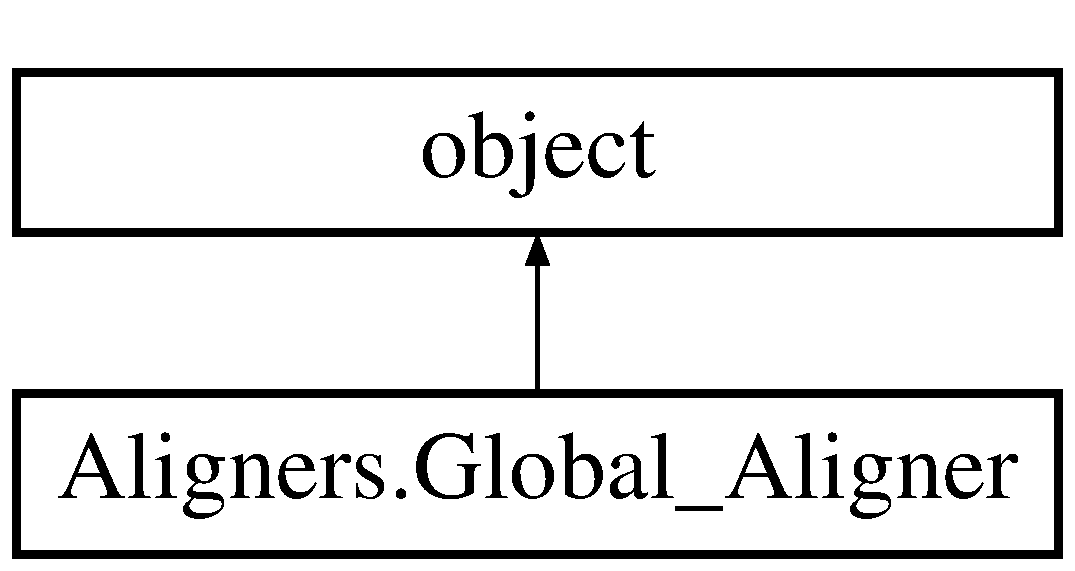
\includegraphics[height=2.000000cm]{class_aligners_1_1_global___aligner}
\end{center}
\end{figure}
\subsection*{Public Member Functions}
\begin{DoxyCompactItemize}
\item 
def \hyperlink{class_aligners_1_1_global___aligner_a0ee9494eaed0fec52d8c2c1c95fc646d}{\+\_\+\+\_\+init\+\_\+\+\_\+} (self, \hyperlink{class_aligners_1_1_global___aligner_a04780fa6727d419f44ce9d577b8b651f}{seq1}, \hyperlink{class_aligners_1_1_global___aligner_a19eaae2895d2246e10543689957a0d36}{seq2}, \hyperlink{class_aligners_1_1_global___aligner_a718075378ef694647d0f4c42ecb7adf9}{substitution\+\_\+matrix}, \hyperlink{class_aligners_1_1_global___aligner_a2dccafe7e89339e5b1e7354de601c2cb}{penalty}, \hyperlink{class_aligners_1_1_global___aligner_aa5a4464984be91c2a0407719a1c1a85d}{ext\+\_\+penalty}=None)
\item 
def \hyperlink{class_aligners_1_1_global___aligner_ae3a7749813381c746e7d3245efbfd0de}{get\+\_\+global\+\_\+matrix} (self)
\item 
def \hyperlink{class_aligners_1_1_global___aligner_ae7b1909e0e0262127f767691b20b82e0}{get\+\_\+global\+\_\+alignment} (self)
\end{DoxyCompactItemize}
\subsection*{Public Attributes}
\begin{DoxyCompactItemize}
\item 
\hyperlink{class_aligners_1_1_global___aligner_a04780fa6727d419f44ce9d577b8b651f}{seq1}
\item 
\hyperlink{class_aligners_1_1_global___aligner_a19eaae2895d2246e10543689957a0d36}{seq2}
\item 
\hyperlink{class_aligners_1_1_global___aligner_a2dccafe7e89339e5b1e7354de601c2cb}{penalty}
\item 
\hyperlink{class_aligners_1_1_global___aligner_aa5a4464984be91c2a0407719a1c1a85d}{ext\+\_\+penalty}
\item 
\hyperlink{class_aligners_1_1_global___aligner_a718075378ef694647d0f4c42ecb7adf9}{substitution\+\_\+matrix}
\end{DoxyCompactItemize}


\subsection{Detailed Description}
\begin{DoxyVerb}Class Global_Aligner is created to build a global alignment
scoring matrix and make a global alignment of two sequences
of amino acids with linear or affine gap penalty.
(If linear one needed do not fill in the last argument)
\end{DoxyVerb}
 

\subsection{Constructor \& Destructor Documentation}
\mbox{\Hypertarget{class_aligners_1_1_global___aligner_a0ee9494eaed0fec52d8c2c1c95fc646d}\label{class_aligners_1_1_global___aligner_a0ee9494eaed0fec52d8c2c1c95fc646d}} 
\index{Aligners\+::\+Global\+\_\+\+Aligner@{Aligners\+::\+Global\+\_\+\+Aligner}!\+\_\+\+\_\+init\+\_\+\+\_\+@{\+\_\+\+\_\+init\+\_\+\+\_\+}}
\index{\+\_\+\+\_\+init\+\_\+\+\_\+@{\+\_\+\+\_\+init\+\_\+\+\_\+}!Aligners\+::\+Global\+\_\+\+Aligner@{Aligners\+::\+Global\+\_\+\+Aligner}}
\subsubsection{\texorpdfstring{\+\_\+\+\_\+init\+\_\+\+\_\+()}{\_\_init\_\_()}}
{\footnotesize\ttfamily def Aligners.\+Global\+\_\+\+Aligner.\+\_\+\+\_\+init\+\_\+\+\_\+ (\begin{DoxyParamCaption}\item[{}]{self,  }\item[{}]{seq1,  }\item[{}]{seq2,  }\item[{}]{substitution\+\_\+matrix,  }\item[{}]{penalty,  }\item[{}]{ext\+\_\+penalty = {\ttfamily None} }\end{DoxyParamCaption})}



\subsection{Member Function Documentation}
\mbox{\Hypertarget{class_aligners_1_1_global___aligner_ae7b1909e0e0262127f767691b20b82e0}\label{class_aligners_1_1_global___aligner_ae7b1909e0e0262127f767691b20b82e0}} 
\index{Aligners\+::\+Global\+\_\+\+Aligner@{Aligners\+::\+Global\+\_\+\+Aligner}!get\+\_\+global\+\_\+alignment@{get\+\_\+global\+\_\+alignment}}
\index{get\+\_\+global\+\_\+alignment@{get\+\_\+global\+\_\+alignment}!Aligners\+::\+Global\+\_\+\+Aligner@{Aligners\+::\+Global\+\_\+\+Aligner}}
\subsubsection{\texorpdfstring{get\+\_\+global\+\_\+alignment()}{get\_global\_alignment()}}
{\footnotesize\ttfamily def Aligners.\+Global\+\_\+\+Aligner.\+get\+\_\+global\+\_\+alignment (\begin{DoxyParamCaption}\item[{}]{self }\end{DoxyParamCaption})}

\begin{DoxyVerb}global alignment of two sequences. Returns a tuple
(align-seq1, align-seq2, align-score)
\end{DoxyVerb}
 \mbox{\Hypertarget{class_aligners_1_1_global___aligner_ae3a7749813381c746e7d3245efbfd0de}\label{class_aligners_1_1_global___aligner_ae3a7749813381c746e7d3245efbfd0de}} 
\index{Aligners\+::\+Global\+\_\+\+Aligner@{Aligners\+::\+Global\+\_\+\+Aligner}!get\+\_\+global\+\_\+matrix@{get\+\_\+global\+\_\+matrix}}
\index{get\+\_\+global\+\_\+matrix@{get\+\_\+global\+\_\+matrix}!Aligners\+::\+Global\+\_\+\+Aligner@{Aligners\+::\+Global\+\_\+\+Aligner}}
\subsubsection{\texorpdfstring{get\+\_\+global\+\_\+matrix()}{get\_global\_matrix()}}
{\footnotesize\ttfamily def Aligners.\+Global\+\_\+\+Aligner.\+get\+\_\+global\+\_\+matrix (\begin{DoxyParamCaption}\item[{}]{self }\end{DoxyParamCaption})}

\begin{DoxyVerb}building a global alignment scoring matrix\end{DoxyVerb}
 

\subsection{Member Data Documentation}
\mbox{\Hypertarget{class_aligners_1_1_global___aligner_aa5a4464984be91c2a0407719a1c1a85d}\label{class_aligners_1_1_global___aligner_aa5a4464984be91c2a0407719a1c1a85d}} 
\index{Aligners\+::\+Global\+\_\+\+Aligner@{Aligners\+::\+Global\+\_\+\+Aligner}!ext\+\_\+penalty@{ext\+\_\+penalty}}
\index{ext\+\_\+penalty@{ext\+\_\+penalty}!Aligners\+::\+Global\+\_\+\+Aligner@{Aligners\+::\+Global\+\_\+\+Aligner}}
\subsubsection{\texorpdfstring{ext\+\_\+penalty}{ext\_penalty}}
{\footnotesize\ttfamily Aligners.\+Global\+\_\+\+Aligner.\+ext\+\_\+penalty}

\mbox{\Hypertarget{class_aligners_1_1_global___aligner_a2dccafe7e89339e5b1e7354de601c2cb}\label{class_aligners_1_1_global___aligner_a2dccafe7e89339e5b1e7354de601c2cb}} 
\index{Aligners\+::\+Global\+\_\+\+Aligner@{Aligners\+::\+Global\+\_\+\+Aligner}!penalty@{penalty}}
\index{penalty@{penalty}!Aligners\+::\+Global\+\_\+\+Aligner@{Aligners\+::\+Global\+\_\+\+Aligner}}
\subsubsection{\texorpdfstring{penalty}{penalty}}
{\footnotesize\ttfamily Aligners.\+Global\+\_\+\+Aligner.\+penalty}

\mbox{\Hypertarget{class_aligners_1_1_global___aligner_a04780fa6727d419f44ce9d577b8b651f}\label{class_aligners_1_1_global___aligner_a04780fa6727d419f44ce9d577b8b651f}} 
\index{Aligners\+::\+Global\+\_\+\+Aligner@{Aligners\+::\+Global\+\_\+\+Aligner}!seq1@{seq1}}
\index{seq1@{seq1}!Aligners\+::\+Global\+\_\+\+Aligner@{Aligners\+::\+Global\+\_\+\+Aligner}}
\subsubsection{\texorpdfstring{seq1}{seq1}}
{\footnotesize\ttfamily Aligners.\+Global\+\_\+\+Aligner.\+seq1}

\mbox{\Hypertarget{class_aligners_1_1_global___aligner_a19eaae2895d2246e10543689957a0d36}\label{class_aligners_1_1_global___aligner_a19eaae2895d2246e10543689957a0d36}} 
\index{Aligners\+::\+Global\+\_\+\+Aligner@{Aligners\+::\+Global\+\_\+\+Aligner}!seq2@{seq2}}
\index{seq2@{seq2}!Aligners\+::\+Global\+\_\+\+Aligner@{Aligners\+::\+Global\+\_\+\+Aligner}}
\subsubsection{\texorpdfstring{seq2}{seq2}}
{\footnotesize\ttfamily Aligners.\+Global\+\_\+\+Aligner.\+seq2}

\mbox{\Hypertarget{class_aligners_1_1_global___aligner_a718075378ef694647d0f4c42ecb7adf9}\label{class_aligners_1_1_global___aligner_a718075378ef694647d0f4c42ecb7adf9}} 
\index{Aligners\+::\+Global\+\_\+\+Aligner@{Aligners\+::\+Global\+\_\+\+Aligner}!substitution\+\_\+matrix@{substitution\+\_\+matrix}}
\index{substitution\+\_\+matrix@{substitution\+\_\+matrix}!Aligners\+::\+Global\+\_\+\+Aligner@{Aligners\+::\+Global\+\_\+\+Aligner}}
\subsubsection{\texorpdfstring{substitution\+\_\+matrix}{substitution\_matrix}}
{\footnotesize\ttfamily Aligners.\+Global\+\_\+\+Aligner.\+substitution\+\_\+matrix}



The documentation for this class was generated from the following file\+:\begin{DoxyCompactItemize}
\item 
/\+Users/ed/dev/mm/aligner/\hyperlink{_aligners_8py}{Aligners.\+py}\end{DoxyCompactItemize}

\hypertarget{class_aligners_1_1_local___aligner}{}\section{Aligners.\+Local\+\_\+\+Aligner Class Reference}
\label{class_aligners_1_1_local___aligner}\index{Aligners.\+Local\+\_\+\+Aligner@{Aligners.\+Local\+\_\+\+Aligner}}
Inheritance diagram for Aligners.\+Local\+\_\+\+Aligner\+:\begin{figure}[H]
\begin{center}
\leavevmode
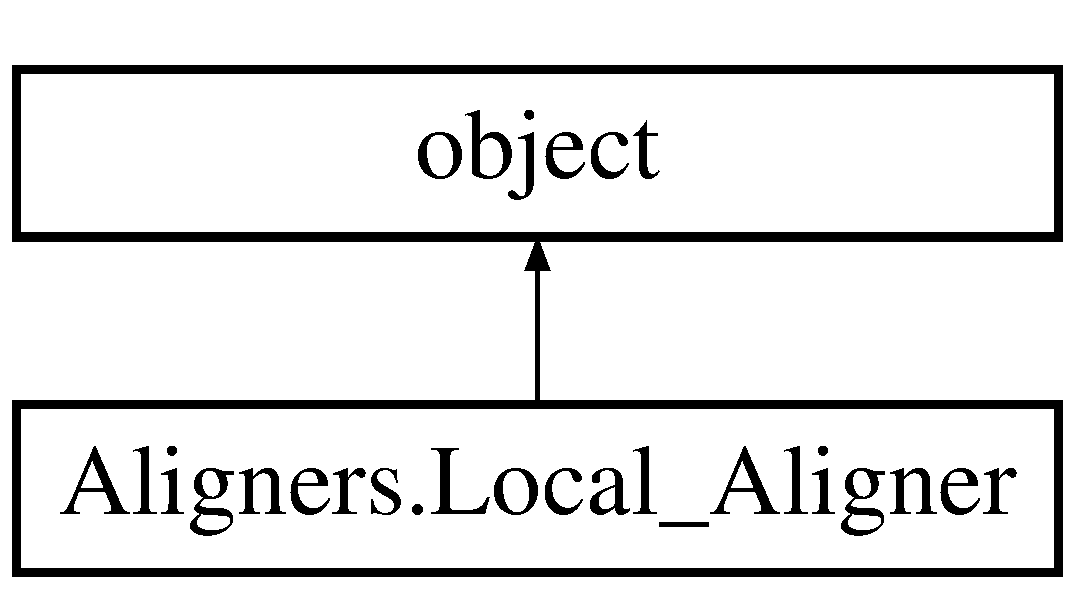
\includegraphics[height=2.000000cm]{class_aligners_1_1_local___aligner}
\end{center}
\end{figure}
\subsection*{Public Member Functions}
\begin{DoxyCompactItemize}
\item 
def \hyperlink{class_aligners_1_1_local___aligner_abbe736e7f3e06b702a844384a1fe85b6}{\+\_\+\+\_\+init\+\_\+\+\_\+} (self, \hyperlink{class_aligners_1_1_local___aligner_a285806896f5d284119dfa1f63792c45e}{seq1}, \hyperlink{class_aligners_1_1_local___aligner_af0ce861edb14e519aa5cda0dbd50600c}{seq2}, \hyperlink{class_aligners_1_1_local___aligner_a6ea6deadde6b8207bfb2c001c4bb3f42}{substitution\+\_\+matrix}, \hyperlink{class_aligners_1_1_local___aligner_aa41272a04dd3ec9ca9e9dcecc6fd2566}{penalty}, \hyperlink{class_aligners_1_1_local___aligner_aa7d238d0b57edc861e02b0b39c8fb7f1}{ext\+\_\+penalty}=None)
\item 
def \hyperlink{class_aligners_1_1_local___aligner_a2df499a9d5f9b3cbae94999687bc7a5d}{get\+\_\+local\+\_\+matrix} (self)
\item 
def \hyperlink{class_aligners_1_1_local___aligner_ad7c960fc046613632da34db5857e4c19}{get\+\_\+local\+\_\+alignment} (self)
\end{DoxyCompactItemize}
\subsection*{Public Attributes}
\begin{DoxyCompactItemize}
\item 
\hyperlink{class_aligners_1_1_local___aligner_a285806896f5d284119dfa1f63792c45e}{seq1}
\item 
\hyperlink{class_aligners_1_1_local___aligner_af0ce861edb14e519aa5cda0dbd50600c}{seq2}
\item 
\hyperlink{class_aligners_1_1_local___aligner_aa41272a04dd3ec9ca9e9dcecc6fd2566}{penalty}
\item 
\hyperlink{class_aligners_1_1_local___aligner_aa7d238d0b57edc861e02b0b39c8fb7f1}{ext\+\_\+penalty}
\item 
\hyperlink{class_aligners_1_1_local___aligner_a6ea6deadde6b8207bfb2c001c4bb3f42}{substitution\+\_\+matrix}
\end{DoxyCompactItemize}


\subsection{Detailed Description}
\begin{DoxyVerb}Class Local_Aligner is created to build a local alignment scoring matrix
and make a local alignment of two sequences of amino acids
with linear or affine gap penalty.
(If linear one needed do not fill in the last argument)
\end{DoxyVerb}
 

\subsection{Constructor \& Destructor Documentation}
\mbox{\Hypertarget{class_aligners_1_1_local___aligner_abbe736e7f3e06b702a844384a1fe85b6}\label{class_aligners_1_1_local___aligner_abbe736e7f3e06b702a844384a1fe85b6}} 
\index{Aligners\+::\+Local\+\_\+\+Aligner@{Aligners\+::\+Local\+\_\+\+Aligner}!\+\_\+\+\_\+init\+\_\+\+\_\+@{\+\_\+\+\_\+init\+\_\+\+\_\+}}
\index{\+\_\+\+\_\+init\+\_\+\+\_\+@{\+\_\+\+\_\+init\+\_\+\+\_\+}!Aligners\+::\+Local\+\_\+\+Aligner@{Aligners\+::\+Local\+\_\+\+Aligner}}
\subsubsection{\texorpdfstring{\+\_\+\+\_\+init\+\_\+\+\_\+()}{\_\_init\_\_()}}
{\footnotesize\ttfamily def Aligners.\+Local\+\_\+\+Aligner.\+\_\+\+\_\+init\+\_\+\+\_\+ (\begin{DoxyParamCaption}\item[{}]{self,  }\item[{}]{seq1,  }\item[{}]{seq2,  }\item[{}]{substitution\+\_\+matrix,  }\item[{}]{penalty,  }\item[{}]{ext\+\_\+penalty = {\ttfamily None} }\end{DoxyParamCaption})}



\subsection{Member Function Documentation}
\mbox{\Hypertarget{class_aligners_1_1_local___aligner_ad7c960fc046613632da34db5857e4c19}\label{class_aligners_1_1_local___aligner_ad7c960fc046613632da34db5857e4c19}} 
\index{Aligners\+::\+Local\+\_\+\+Aligner@{Aligners\+::\+Local\+\_\+\+Aligner}!get\+\_\+local\+\_\+alignment@{get\+\_\+local\+\_\+alignment}}
\index{get\+\_\+local\+\_\+alignment@{get\+\_\+local\+\_\+alignment}!Aligners\+::\+Local\+\_\+\+Aligner@{Aligners\+::\+Local\+\_\+\+Aligner}}
\subsubsection{\texorpdfstring{get\+\_\+local\+\_\+alignment()}{get\_local\_alignment()}}
{\footnotesize\ttfamily def Aligners.\+Local\+\_\+\+Aligner.\+get\+\_\+local\+\_\+alignment (\begin{DoxyParamCaption}\item[{}]{self }\end{DoxyParamCaption})}

\begin{DoxyVerb}local alignment of two sequences. Returns a tuple
(align-seq1, align-seq2, align-score)
\end{DoxyVerb}
 \mbox{\Hypertarget{class_aligners_1_1_local___aligner_a2df499a9d5f9b3cbae94999687bc7a5d}\label{class_aligners_1_1_local___aligner_a2df499a9d5f9b3cbae94999687bc7a5d}} 
\index{Aligners\+::\+Local\+\_\+\+Aligner@{Aligners\+::\+Local\+\_\+\+Aligner}!get\+\_\+local\+\_\+matrix@{get\+\_\+local\+\_\+matrix}}
\index{get\+\_\+local\+\_\+matrix@{get\+\_\+local\+\_\+matrix}!Aligners\+::\+Local\+\_\+\+Aligner@{Aligners\+::\+Local\+\_\+\+Aligner}}
\subsubsection{\texorpdfstring{get\+\_\+local\+\_\+matrix()}{get\_local\_matrix()}}
{\footnotesize\ttfamily def Aligners.\+Local\+\_\+\+Aligner.\+get\+\_\+local\+\_\+matrix (\begin{DoxyParamCaption}\item[{}]{self }\end{DoxyParamCaption})}

\begin{DoxyVerb}building a global alignment scoring matrix\end{DoxyVerb}
 

\subsection{Member Data Documentation}
\mbox{\Hypertarget{class_aligners_1_1_local___aligner_aa7d238d0b57edc861e02b0b39c8fb7f1}\label{class_aligners_1_1_local___aligner_aa7d238d0b57edc861e02b0b39c8fb7f1}} 
\index{Aligners\+::\+Local\+\_\+\+Aligner@{Aligners\+::\+Local\+\_\+\+Aligner}!ext\+\_\+penalty@{ext\+\_\+penalty}}
\index{ext\+\_\+penalty@{ext\+\_\+penalty}!Aligners\+::\+Local\+\_\+\+Aligner@{Aligners\+::\+Local\+\_\+\+Aligner}}
\subsubsection{\texorpdfstring{ext\+\_\+penalty}{ext\_penalty}}
{\footnotesize\ttfamily Aligners.\+Local\+\_\+\+Aligner.\+ext\+\_\+penalty}

\mbox{\Hypertarget{class_aligners_1_1_local___aligner_aa41272a04dd3ec9ca9e9dcecc6fd2566}\label{class_aligners_1_1_local___aligner_aa41272a04dd3ec9ca9e9dcecc6fd2566}} 
\index{Aligners\+::\+Local\+\_\+\+Aligner@{Aligners\+::\+Local\+\_\+\+Aligner}!penalty@{penalty}}
\index{penalty@{penalty}!Aligners\+::\+Local\+\_\+\+Aligner@{Aligners\+::\+Local\+\_\+\+Aligner}}
\subsubsection{\texorpdfstring{penalty}{penalty}}
{\footnotesize\ttfamily Aligners.\+Local\+\_\+\+Aligner.\+penalty}

\mbox{\Hypertarget{class_aligners_1_1_local___aligner_a285806896f5d284119dfa1f63792c45e}\label{class_aligners_1_1_local___aligner_a285806896f5d284119dfa1f63792c45e}} 
\index{Aligners\+::\+Local\+\_\+\+Aligner@{Aligners\+::\+Local\+\_\+\+Aligner}!seq1@{seq1}}
\index{seq1@{seq1}!Aligners\+::\+Local\+\_\+\+Aligner@{Aligners\+::\+Local\+\_\+\+Aligner}}
\subsubsection{\texorpdfstring{seq1}{seq1}}
{\footnotesize\ttfamily Aligners.\+Local\+\_\+\+Aligner.\+seq1}

\mbox{\Hypertarget{class_aligners_1_1_local___aligner_af0ce861edb14e519aa5cda0dbd50600c}\label{class_aligners_1_1_local___aligner_af0ce861edb14e519aa5cda0dbd50600c}} 
\index{Aligners\+::\+Local\+\_\+\+Aligner@{Aligners\+::\+Local\+\_\+\+Aligner}!seq2@{seq2}}
\index{seq2@{seq2}!Aligners\+::\+Local\+\_\+\+Aligner@{Aligners\+::\+Local\+\_\+\+Aligner}}
\subsubsection{\texorpdfstring{seq2}{seq2}}
{\footnotesize\ttfamily Aligners.\+Local\+\_\+\+Aligner.\+seq2}

\mbox{\Hypertarget{class_aligners_1_1_local___aligner_a6ea6deadde6b8207bfb2c001c4bb3f42}\label{class_aligners_1_1_local___aligner_a6ea6deadde6b8207bfb2c001c4bb3f42}} 
\index{Aligners\+::\+Local\+\_\+\+Aligner@{Aligners\+::\+Local\+\_\+\+Aligner}!substitution\+\_\+matrix@{substitution\+\_\+matrix}}
\index{substitution\+\_\+matrix@{substitution\+\_\+matrix}!Aligners\+::\+Local\+\_\+\+Aligner@{Aligners\+::\+Local\+\_\+\+Aligner}}
\subsubsection{\texorpdfstring{substitution\+\_\+matrix}{substitution\_matrix}}
{\footnotesize\ttfamily Aligners.\+Local\+\_\+\+Aligner.\+substitution\+\_\+matrix}



The documentation for this class was generated from the following file\+:\begin{DoxyCompactItemize}
\item 
/\+Users/ed/dev/mm/aligner/\hyperlink{_aligners_8py}{Aligners.\+py}\end{DoxyCompactItemize}

\hypertarget{class_substitution___matrix_1_1_substitution___matrix}{}\section{Substitution\+\_\+\+Matrix.\+Substitution\+\_\+\+Matrix Class Reference}
\label{class_substitution___matrix_1_1_substitution___matrix}\index{Substitution\+\_\+\+Matrix.\+Substitution\+\_\+\+Matrix@{Substitution\+\_\+\+Matrix.\+Substitution\+\_\+\+Matrix}}
Inheritance diagram for Substitution\+\_\+\+Matrix.\+Substitution\+\_\+\+Matrix\+:\begin{figure}[H]
\begin{center}
\leavevmode
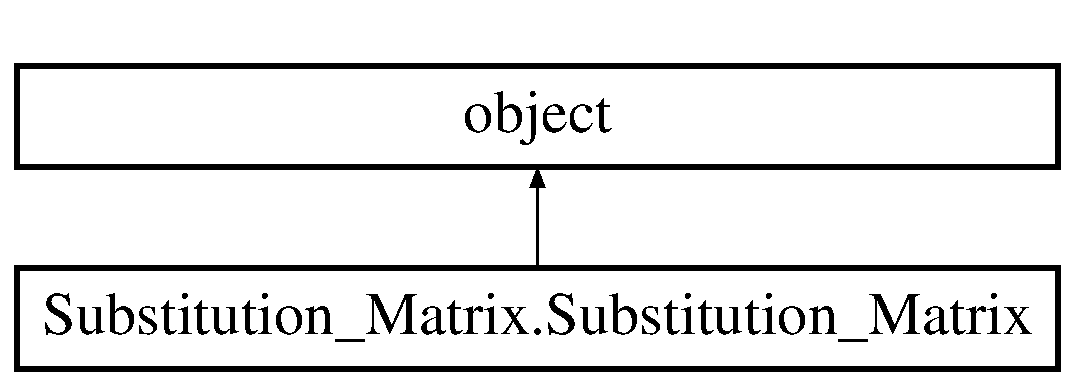
\includegraphics[height=2.000000cm]{class_substitution___matrix_1_1_substitution___matrix}
\end{center}
\end{figure}
\subsection*{Public Member Functions}
\begin{DoxyCompactItemize}
\item 
def \hyperlink{class_substitution___matrix_1_1_substitution___matrix_adce790552ac5e28f1176df6eee08ea41}{\+\_\+\+\_\+init\+\_\+\+\_\+} (self, \hyperlink{class_substitution___matrix_1_1_substitution___matrix_a0efcbb6cff66f7bc445ba6f8eee16db4}{matrix\+\_\+name})
\item 
def \hyperlink{class_substitution___matrix_1_1_substitution___matrix_ac1c1ba4d51ec687cb13b09faef89820d}{get\+\_\+substitution\+\_\+value} (self, acid1, acid2)
\item 
def \hyperlink{class_substitution___matrix_1_1_substitution___matrix_ade8bcf1a7cb67967777fe0603ea8383b}{\+\_\+\+\_\+str\+\_\+\+\_\+} (self)
\end{DoxyCompactItemize}
\subsection*{Public Attributes}
\begin{DoxyCompactItemize}
\item 
\hyperlink{class_substitution___matrix_1_1_substitution___matrix_a0efcbb6cff66f7bc445ba6f8eee16db4}{matrix\+\_\+name}
\item 
\hyperlink{class_substitution___matrix_1_1_substitution___matrix_a700c5a4bca5bbe99e8f7d0d66b1cb8e8}{url}
\item 
\hyperlink{class_substitution___matrix_1_1_substitution___matrix_ab77bb34d48cccce60c0377053e415eb0}{matrix\+\_\+full}
\end{DoxyCompactItemize}


\subsection{Detailed Description}
\begin{DoxyVerb}Class Substitution_Matrix is created to parse and store
Substitution Matrixes (PAM, Blosum) from mbio.ncsu.edu
and check substitution values of amino acids
\end{DoxyVerb}
 

\subsection{Constructor \& Destructor Documentation}
\mbox{\Hypertarget{class_substitution___matrix_1_1_substitution___matrix_adce790552ac5e28f1176df6eee08ea41}\label{class_substitution___matrix_1_1_substitution___matrix_adce790552ac5e28f1176df6eee08ea41}} 
\index{Substitution\+\_\+\+Matrix\+::\+Substitution\+\_\+\+Matrix@{Substitution\+\_\+\+Matrix\+::\+Substitution\+\_\+\+Matrix}!\+\_\+\+\_\+init\+\_\+\+\_\+@{\+\_\+\+\_\+init\+\_\+\+\_\+}}
\index{\+\_\+\+\_\+init\+\_\+\+\_\+@{\+\_\+\+\_\+init\+\_\+\+\_\+}!Substitution\+\_\+\+Matrix\+::\+Substitution\+\_\+\+Matrix@{Substitution\+\_\+\+Matrix\+::\+Substitution\+\_\+\+Matrix}}
\subsubsection{\texorpdfstring{\+\_\+\+\_\+init\+\_\+\+\_\+()}{\_\_init\_\_()}}
{\footnotesize\ttfamily def Substitution\+\_\+\+Matrix.\+Substitution\+\_\+\+Matrix.\+\_\+\+\_\+init\+\_\+\+\_\+ (\begin{DoxyParamCaption}\item[{}]{self,  }\item[{}]{matrix\+\_\+name }\end{DoxyParamCaption})}



\subsection{Member Function Documentation}
\mbox{\Hypertarget{class_substitution___matrix_1_1_substitution___matrix_ade8bcf1a7cb67967777fe0603ea8383b}\label{class_substitution___matrix_1_1_substitution___matrix_ade8bcf1a7cb67967777fe0603ea8383b}} 
\index{Substitution\+\_\+\+Matrix\+::\+Substitution\+\_\+\+Matrix@{Substitution\+\_\+\+Matrix\+::\+Substitution\+\_\+\+Matrix}!\+\_\+\+\_\+str\+\_\+\+\_\+@{\+\_\+\+\_\+str\+\_\+\+\_\+}}
\index{\+\_\+\+\_\+str\+\_\+\+\_\+@{\+\_\+\+\_\+str\+\_\+\+\_\+}!Substitution\+\_\+\+Matrix\+::\+Substitution\+\_\+\+Matrix@{Substitution\+\_\+\+Matrix\+::\+Substitution\+\_\+\+Matrix}}
\subsubsection{\texorpdfstring{\+\_\+\+\_\+str\+\_\+\+\_\+()}{\_\_str\_\_()}}
{\footnotesize\ttfamily def Substitution\+\_\+\+Matrix.\+Substitution\+\_\+\+Matrix.\+\_\+\+\_\+str\+\_\+\+\_\+ (\begin{DoxyParamCaption}\item[{}]{self }\end{DoxyParamCaption})}

\mbox{\Hypertarget{class_substitution___matrix_1_1_substitution___matrix_ac1c1ba4d51ec687cb13b09faef89820d}\label{class_substitution___matrix_1_1_substitution___matrix_ac1c1ba4d51ec687cb13b09faef89820d}} 
\index{Substitution\+\_\+\+Matrix\+::\+Substitution\+\_\+\+Matrix@{Substitution\+\_\+\+Matrix\+::\+Substitution\+\_\+\+Matrix}!get\+\_\+substitution\+\_\+value@{get\+\_\+substitution\+\_\+value}}
\index{get\+\_\+substitution\+\_\+value@{get\+\_\+substitution\+\_\+value}!Substitution\+\_\+\+Matrix\+::\+Substitution\+\_\+\+Matrix@{Substitution\+\_\+\+Matrix\+::\+Substitution\+\_\+\+Matrix}}
\subsubsection{\texorpdfstring{get\+\_\+substitution\+\_\+value()}{get\_substitution\_value()}}
{\footnotesize\ttfamily def Substitution\+\_\+\+Matrix.\+Substitution\+\_\+\+Matrix.\+get\+\_\+substitution\+\_\+value (\begin{DoxyParamCaption}\item[{}]{self,  }\item[{}]{acid1,  }\item[{}]{acid2 }\end{DoxyParamCaption})}

\begin{DoxyVerb}allows to check alignment value for two amino acids
based on chosen substitution matrix
\end{DoxyVerb}
 

\subsection{Member Data Documentation}
\mbox{\Hypertarget{class_substitution___matrix_1_1_substitution___matrix_ab77bb34d48cccce60c0377053e415eb0}\label{class_substitution___matrix_1_1_substitution___matrix_ab77bb34d48cccce60c0377053e415eb0}} 
\index{Substitution\+\_\+\+Matrix\+::\+Substitution\+\_\+\+Matrix@{Substitution\+\_\+\+Matrix\+::\+Substitution\+\_\+\+Matrix}!matrix\+\_\+full@{matrix\+\_\+full}}
\index{matrix\+\_\+full@{matrix\+\_\+full}!Substitution\+\_\+\+Matrix\+::\+Substitution\+\_\+\+Matrix@{Substitution\+\_\+\+Matrix\+::\+Substitution\+\_\+\+Matrix}}
\subsubsection{\texorpdfstring{matrix\+\_\+full}{matrix\_full}}
{\footnotesize\ttfamily Substitution\+\_\+\+Matrix.\+Substitution\+\_\+\+Matrix.\+matrix\+\_\+full}

\mbox{\Hypertarget{class_substitution___matrix_1_1_substitution___matrix_a0efcbb6cff66f7bc445ba6f8eee16db4}\label{class_substitution___matrix_1_1_substitution___matrix_a0efcbb6cff66f7bc445ba6f8eee16db4}} 
\index{Substitution\+\_\+\+Matrix\+::\+Substitution\+\_\+\+Matrix@{Substitution\+\_\+\+Matrix\+::\+Substitution\+\_\+\+Matrix}!matrix\+\_\+name@{matrix\+\_\+name}}
\index{matrix\+\_\+name@{matrix\+\_\+name}!Substitution\+\_\+\+Matrix\+::\+Substitution\+\_\+\+Matrix@{Substitution\+\_\+\+Matrix\+::\+Substitution\+\_\+\+Matrix}}
\subsubsection{\texorpdfstring{matrix\+\_\+name}{matrix\_name}}
{\footnotesize\ttfamily Substitution\+\_\+\+Matrix.\+Substitution\+\_\+\+Matrix.\+matrix\+\_\+name}

\mbox{\Hypertarget{class_substitution___matrix_1_1_substitution___matrix_a700c5a4bca5bbe99e8f7d0d66b1cb8e8}\label{class_substitution___matrix_1_1_substitution___matrix_a700c5a4bca5bbe99e8f7d0d66b1cb8e8}} 
\index{Substitution\+\_\+\+Matrix\+::\+Substitution\+\_\+\+Matrix@{Substitution\+\_\+\+Matrix\+::\+Substitution\+\_\+\+Matrix}!url@{url}}
\index{url@{url}!Substitution\+\_\+\+Matrix\+::\+Substitution\+\_\+\+Matrix@{Substitution\+\_\+\+Matrix\+::\+Substitution\+\_\+\+Matrix}}
\subsubsection{\texorpdfstring{url}{url}}
{\footnotesize\ttfamily Substitution\+\_\+\+Matrix.\+Substitution\+\_\+\+Matrix.\+url}



The documentation for this class was generated from the following file\+:\begin{DoxyCompactItemize}
\item 
/\+Users/ed/dev/mm/aligner/\hyperlink{_substitution___matrix_8py}{Substitution\+\_\+\+Matrix.\+py}\end{DoxyCompactItemize}

\chapter{File Documentation}
\hypertarget{_aligners_8py}{}\section{/\+Users/ed/dev/mm/aligner/\+Aligners.py File Reference}
\label{_aligners_8py}\index{/\+Users/ed/dev/mm/aligner/\+Aligners.\+py@{/\+Users/ed/dev/mm/aligner/\+Aligners.\+py}}
\subsection*{Classes}
\begin{DoxyCompactItemize}
\item 
class \hyperlink{class_aligners_1_1_global___aligner}{Aligners.\+Global\+\_\+\+Aligner}
\item 
class \hyperlink{class_aligners_1_1_local___aligner}{Aligners.\+Local\+\_\+\+Aligner}
\end{DoxyCompactItemize}
\subsection*{Namespaces}
\begin{DoxyCompactItemize}
\item 
 \hyperlink{namespace_aligners}{Aligners}
\end{DoxyCompactItemize}

\hypertarget{_main_8py}{}\section{/\+Users/ed/dev/mm/aligner/\+Main.py File Reference}
\label{_main_8py}\index{/\+Users/ed/dev/mm/aligner/\+Main.\+py@{/\+Users/ed/dev/mm/aligner/\+Main.\+py}}
\subsection*{Namespaces}
\begin{DoxyCompactItemize}
\item 
 \hyperlink{namespace_main}{Main}
\end{DoxyCompactItemize}
\subsection*{Functions}
\begin{DoxyCompactItemize}
\item 
def \hyperlink{namespace_main_a5e2b1a2a697c8ff97fe0508423af05f2}{Main.\+get\+\_\+sequences} (file)
\end{DoxyCompactItemize}
\subsection*{Variables}
\begin{DoxyCompactItemize}
\item 
def \hyperlink{namespace_main_a0f7dfdcfc82e28e54d2d9b4355d51c6a}{Main.\+protein\+\_\+sequences} = get\+\_\+sequences(\textquotesingle{}protein-\/sequences.\+fasta\textquotesingle{})
\item 
def \hyperlink{namespace_main_ad0e687821118d10a87cd81cdb0597636}{Main.\+ww\+\_\+sequences} = get\+\_\+sequences(\textquotesingle{}WW-\/sequence.\+fasta\textquotesingle{})
\item 
\hyperlink{namespace_main_a027017501a6249c536a21b55ab4ff57d}{Main.\+global\+\_\+test} = Global\+\_\+\+Aligner(ww\+\_\+sequences\mbox{[}1\mbox{]}\mbox{[}0\mbox{]}, ww\+\_\+sequences\mbox{[}1\mbox{]}\mbox{[}1\mbox{]}, pam250, -\/8, -\/3)
\item 
\hyperlink{namespace_main_a855511465ef4b71860406d664b6b7f61}{Main.\+local\+\_\+test} = Local\+\_\+\+Aligner(protein\+\_\+sequences\mbox{[}1\mbox{]}\mbox{[}0\mbox{]}, protein\+\_\+sequences\mbox{[}1\mbox{]}\mbox{[}3\mbox{]}, pam120, -\/10, -\/2)
\end{DoxyCompactItemize}

\hypertarget{_substitution___matrix_8py}{}\section{/\+Users/ed/dev/mm/aligner/\+Substitution\+\_\+\+Matrix.py File Reference}
\label{_substitution___matrix_8py}\index{/\+Users/ed/dev/mm/aligner/\+Substitution\+\_\+\+Matrix.\+py@{/\+Users/ed/dev/mm/aligner/\+Substitution\+\_\+\+Matrix.\+py}}
\subsection*{Classes}
\begin{DoxyCompactItemize}
\item 
class \hyperlink{class_substitution___matrix_1_1_substitution___matrix}{Substitution\+\_\+\+Matrix.\+Substitution\+\_\+\+Matrix}
\end{DoxyCompactItemize}
\subsection*{Namespaces}
\begin{DoxyCompactItemize}
\item 
 \hyperlink{namespace_substitution___matrix}{Substitution\+\_\+\+Matrix}
\end{DoxyCompactItemize}
\subsection*{Variables}
\begin{DoxyCompactItemize}
\item 
\hyperlink{namespace_substitution___matrix_a8495f9058eb7997200ab8a476c96c948}{Substitution\+\_\+\+Matrix.\+pam120} = Substitution\+\_\+\+Matrix(\textquotesingle{}P\+A\+M120\textquotesingle{})
\item 
\hyperlink{namespace_substitution___matrix_ad84746b6a1720d01b8648774f1020aa7}{Substitution\+\_\+\+Matrix.\+pam250} = Substitution\+\_\+\+Matrix(\textquotesingle{}P\+A\+M250\textquotesingle{})
\item 
\hyperlink{namespace_substitution___matrix_a9e4911111c065bc2e034165b9ddd1ca8}{Substitution\+\_\+\+Matrix.\+blosum62} = Substitution\+\_\+\+Matrix(\textquotesingle{}B\+L\+O\+S\+U\+M62\textquotesingle{})
\end{DoxyCompactItemize}

%--- End generated contents ---

% Index
\backmatter
\newpage
\phantomsection
\clearemptydoublepage
\addcontentsline{toc}{chapter}{Index}
\printindex

\end{document}
